% ---------------------------------------------------------------------------------------
\chapter{Análisis y Procesamiento de im\'agenes }\label{chap3}


Tanto en la ciencia de datos, commom en estad\'istica, y la compitaci\'on, el an\'alisis de im\'agenes es un ha emergido como un \'area de estudio de gran importancia, que he sido pivotal y con un extenso alcance en multiples discuplinas. De la forma en que la era digital avanza, la cantidad de datos que se generan en forma de im\'agenes es cada vez mayor, y con ello la necesidad herramientas para analizar, procesar, comprender y en general obtener informaci\'on relevante de estas im\'agenes. 

El uso de im\'agenes ha evolucionado de aplicaci\'ones tradicionales como imagenolog\'ia satelital y diagn\'ostico m\'edico, a dominios m\'as modernos como inteligencia artificial, reconocimiento facial, y vehiculos aut\'onomos. La habilidad de detectar patrones, animal\'ias, y derivar informaci\'on de estas tiene un potencial enorme para la innovaci\'on y el desarrollo de nuevas tecnolog\'ias. 

En este cap\'itulo, se introducen los conceptos necesarios para entender el an\'alisis de im\'agenes, y se presentan las herramientas que se utilizaron para el desarrollo de este trabajo. Comenzaremos defininiendo las im\'agenes como matrices, luego presentaremos el banco de im\'agenes a utilizar durante el resto del trabajo, para posteriormente hablar de las caracter\'isticas de una imagen, como el contraste, la luminosidad, y la saturaci\'on. Luego, hablaremos de los espacios de color, y como estos se utilizan para representar una imagen. Finalmente, hablaremos de las t\'ecnicas de comparaci\'on de im\'agenes, en particular como aplicamos t\'ecnicas de comparaci\'on entre vectores sobre im\'agenes,

% ---------------------------------------------------------------------------------------
\section{im\'agenes como matrices}

Una imagen es una representaci\'on visual de un objeto, y se puede definir como una funci\'on bidimensional $f(x,y)$, donde $x$ y $y$ son coordenadas espaciales, y el valor de $f$ en cualquier par de coordenadas $(x,y)$ es la intensidad de la imagen en ese punto. Cuando $x$, $y$, y los valores de intensidad de $f$ son todos finitos y discretos, llamamos a la imagen una imagen digital. En este trabajo hemos utilizado (y seguiremos utilziando) el concepto de imagen digital e imagen de forma intercambiable. Por claridad en notaci\'on y conveniencia, usamos valores enteros para determinar las coordenadas de la imagen, y su origen en la esquina superior izquierda, como se muestra en la siguiente ecuaci\'on:

$$
f(x, y)=\left[\begin{array}{cccc}
f(0,0) & f(0,1) & \cdots & f(0, N-1) \\
f(1,0) & f(1,1) & \cdots & f(1, N-1) \\
\vdots & \vdots & & \vdots \\
f(M-1,0) & f(M-1,1) & \cdots & f(M-1, N-1)
\end{array}\right]
$$

El lado derecho de esta ecuación es una imagen digital representada como un conjunto de números reales. Cada elemento de este conjunto se llama elemento de imagen, píxel o "pel". La Figura \ref{fig:dip_2_18} muestra una representación gráfica de un conjunto de imágenes, donde los ejes $x$ e $y$ se utilizan para denotar las filas y columnas del conjunto. Píxeles específicos son valores del conjunto en un par fijo de coordenadas. Como se mencionó anteriormente, generalmente utilizamos $f(i, j)$ al referirnos a un píxel con coordenadas $(i, j)$.


\begin{figure}[H]
    \centering
    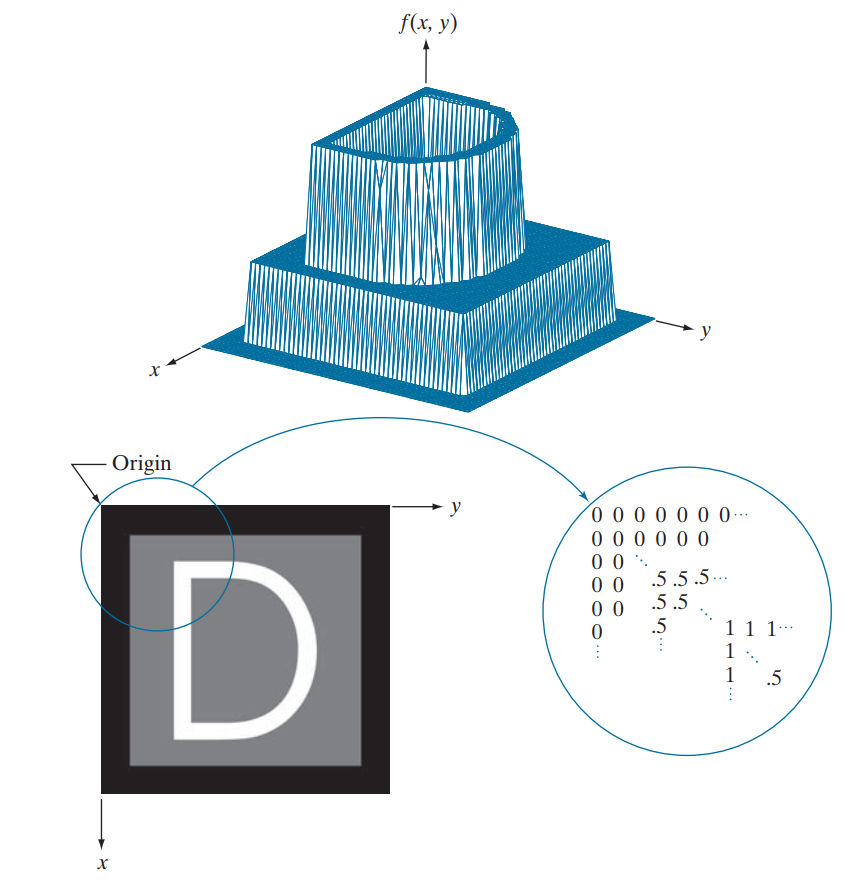
\includegraphics[width=0.6\textwidth]{dip_4_fig2_18.png}
    \caption{
        (a) Imagen representada como una superficie.
        (b) Imagen mostrada como un conjunto de intensidades visuales.
        (c) Imagen presentada como un conjunto numérico en 2D. (Los números 0, 0.6 y 1 representan negro, gris y blanco, respectivamente).}
    \label{fig:dip_2_18}
\end{figure}

Como se ve en la figura \ref{fig:dip_2_18}, y como mencionamos anteriormente, el origen se define en la esquina superior izquierda, esta es una convenci\'on que nace en que mucha tecnolog\'ia usada para representar im\'agenes hacen un barrido de imagen de arriba hacía abajo y de izquierda a derecha, por ejemplo, los televisores. Esto tambi\'en es conveniente dado que concorda con la forma en la que solemos indexar matrices, las cuales tambi\'en podemos podemos utilizar para representar una imagen  de la siguiente forma:

$$
\mathbf{A}=\left[\begin{array}{cccc}
a_{0,0} & a_{0,1} & \cdots & a_{0, N-1} \\
a_{1,0} & a_{1,1} & \cdots & a_{1, N-1} \\
\vdots & \vdots & & \vdots \\
a_{M-1,0} & a_{M-1,1} & \cdots & a_{M-1, N-1}
\end{array}\right]
$$

Normalmente, cuando trabajamos con una imagen obtenida de una c\'amara digital, esta se encuentra en el espacio de color RGB, donde cada pixel de la imagen es representado por tres valores, uno para cada canal de color. Por tanto, podemos representar una imagen RGB como una matriz de $N \times M \times 3$, donde $N$ y $M$ son el ancho y alto de la imagen, y el tercer valor representa los tres canales de color de la siguiente forma:

$$
\mathcal{F}(x, y)=\{R(x, y), G(x, y), B(x, y)\}
$$


Con $R$, $G$, y $B$ representando los valores de los canales rojo, verde y azul respectivamente, y con $x\in[0,M-1]$ e $y\in[0,N-1]$ representando las coordenadas de la imagen. El espacio de color RGB es el espacio m\'as comun para representar im\'agenes en monitores y es como la gran mayoría de c\'amaras digitales capturan im\'agenes, pero no es el \'unico espacio de color que existe, otros ejemplos notables son el espacio CMY (cyan, magenta, yellow) y CMYK (cyan, magenta, yellow, black) son espacios comunmente utilizados en impresi\'on, y el espacio HSI (hue, saturation, intensity), que corresponde de forma cercana a la forma en la que los humanos describimos e interpretamos el color. \cite{DigitalImageProcessing}

Al momento de trabajar con im\'agenes para el contexto de este trabajo, nos es de interes hacerlo con im\'agenes en escala de grises, puesto que queremos mantener la informaci\'on espacial de la imagen, y nos facilitar\'a el calculo m\'as adelante. El paso a escala de grises no es más que un promedio ponderado de los tres canales de color de la imagen, aunque tendría sentido utilizar un promedio simple, la percepción humana varía dependiendo del color, dado que somos mas sensibles a los colores verdes, y menos sensibles a los colores azules. Para esto, podemos convertir una imagen RGB a escala de grises utilizando la siguiente ecuaci\'on:

\begin{equation}
    I(x, y)=0.299 R(x, y)+0.687 G(x, y)+0.114 B(x, y), 
    \label{eq:grayscale}
\end{equation}

que corresponde el canal gris del espacio de colores $YC_bC_r$. En la siguiente figura podemos ver una imagen RGB, una transformaci\'on utilizando un promdeio simple, y su correspondiente imagen en escala de grises como fue definida anteriormente.

\begin{figure}[H]
    \centering
    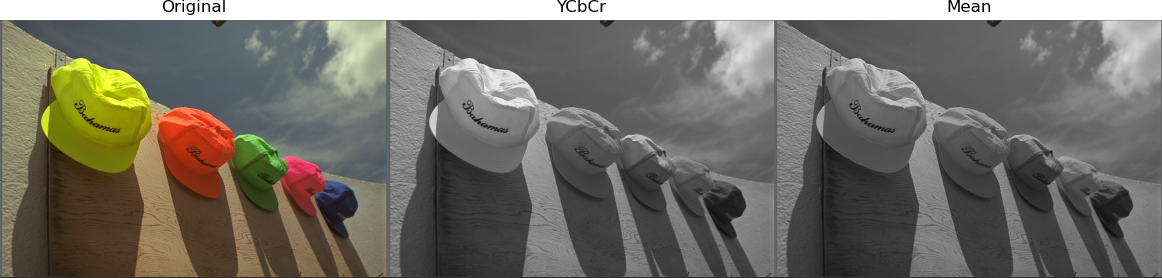
\includegraphics[width=0.8\textwidth]{img_ex_bw.png}
    \caption{Imagen RGB,escala de grises, y promedio simple.}
    \label{fig:rgb2gray}
\end{figure}


\section{Banco de im\'agenes}

El banco que utilizaremos es llamado \textit{Kodak Lossless True Color Image Suite
}\cite{KodakLosslessTrueColorImageSuite} que corresponde a 24 im\'agenes no comprimidas y con color completo, de tama\~no 768x512 pixeles o 512x768 pixeles. Est\'as fueron publicadas por la compa\~nia Eastman Kodak en 1999, y son ampliamente utilizadas en el \'area de procesamiento de im\'agenes. 

Podemos ver las im\'agenes en la figura , y podemos ver las im\'agenes en escala de grises en las firguras \ref{fig:banco_color} y \ref{fig:banco_gris}. Est\'as im\'agenes correponden a una gran variedad de escenas y texturas, teniendo figuras humanas, arquitecura, y paisajes; lo que nos entrega un amplio abanico de posibilidades y variedad al momento de hacer los experimentos.

\begin{figure}[H]
    \centering
    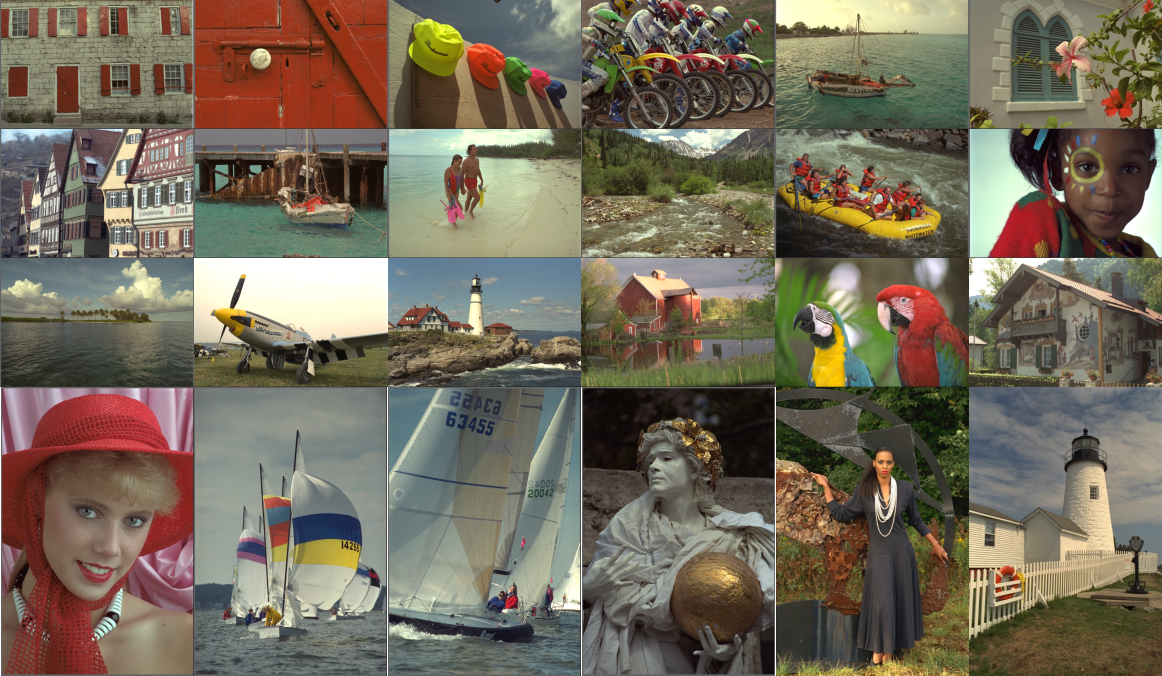
\includegraphics[width=0.8\textwidth]{all_images_grid.png}
    \caption{im\'agenes a utilizar en el banco a color.}
    \label{fig:banco_color}
\end{figure}

\begin{figure}[H]
    \centering
    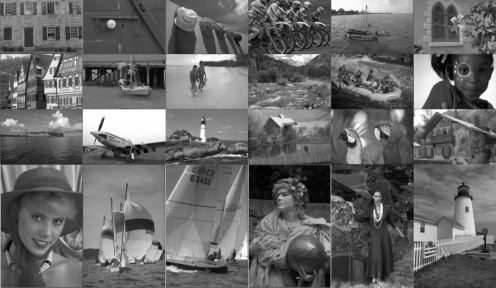
\includegraphics[width=0.8\textwidth]{all_images_grid_bw.png}
    \caption{im\'agenes a utilizar en el banco en escala de grises.}
    \label{fig:banco_gris}
\end{figure}


\section{Comparando im\'agenes}

Cómo discutimos anteriormente, podemos representar una imagen como una matriz de valores, pero esto nos genera un problema al momento de usar los m\'etodos de comparaci\'on descritos en el cap\'itulo \ref{chap3} y \ref{chap4}, puesto que estas est\'an definidas para vectores, y no para matrices. Para solucionar esto, podemos utilizar una de las siguientes dos estrategias:

\subsection{imagen a vector}

La forma m\'as simple de solucionar este problema es convertir la matriz de la imagen en un vector, y luego aplicar los m\'etodos de comparaci\'on sobre este vector. Antes de realizar esta conversi\'on, debemos tener en cuenta problemas generados por esta propuesta. 

La primera es que el m\'etodo que utilizaemos para comparar dos im\'agenes puede no ser agn\'ostico con respecto al orden de los vectores a comparar, lo que nos llevaría a otro problema, la elecci\'on del orden de los elementos del vector. Tenemos la suerte de que todos los m\'etodos de comparaci\'on que utilizaremos son agn\'osticos con respecto al orden de los vectores, por lo que no tendremos que preocuparnos de este problema \cite{Reshef2016} \cite{Szekely2009}.

El segundo problema es la perdida de informaci\'on, esto es dado que cada pixel posee una correlaci\'on espacial con sus pixeles vecinos, y al momento de convertir la matriz en un vector, perdemos esta informaci\'on. Para solucionar esto, podr\'iamos utilizar una curva de Hilbert, que es una curva fractal que se puede utilizar para mapear una matriz en un vector, de forma que los pixeles vecinos en la matriz, sean vecinos en el vector. Sin embargo, esto no es necesario, puesto que los m\'etodos de comparaci\'on que utilizaremos son agn\'osticos con respecto al orden de los vectores.

Por ultimo tenemos un problema de tama\~no, las im\'agenes del banco tienen una resouluci\'on de 512x768, lo que nos genera un vector de 393216 elementos, lo que es un vector de dimensi\'on muy alta, y podr\'ia generar problemas de performance al momento de calcular los coeficientes de comparaci\'on. 

\subsection{Imagen a histograma}

Otra forma de comparar im\'agenes es utilizando un histograma, de la misma forma que en Bicego (2016)\cite{bicego2016} donde, luego de convertir la imagen en escala de grises, cada valor de intensidad corresponde a un bin del histograma, y este es usado para calcular el $\lambda$ optimo para la transformaci\'on de Box-Cox. 

Inspirados en esto, utilizamos los histogramas como un proxy de la imag\'en al momento de realziar la comparaci\'on entre las im\'agenes. Esto tiene el claro beneficio de que el histograma es un vector de dimensi\'on mucho menor que la imagen, y por tanto, el calculo de los coeficientes de comparaci\'on es mucho m\'as r\'apido. Adem\'as en cierta forma estamos manteniendo la informaci\'on espacial de la imagen, puesto que los pixeles vecinos en la imagen, puesto que las intensidades de los pixeles vecinos est\'an relacionadas. 

El claro problema es que dos ima\'agenes pueden tener el mismo histograma, pero ser completamente distintas. Sin embargo, en el contexto de este trabajo, esto no es un problema, puesto que lo que nos interesa es comparar im\'agenes que son similares, puesto que son el resultado de una transformaci\'on de la imagen original.

\section{Ejemplos de comparaci\'on de im\'agenes}

Ya describimos los m\'etodos que usaremos para comprar las im\'agenes usando las t\'ecnicas descritas en el cap\'itulo \ref{chap2} y \ref{chap3}, ahora revisaremos 4 im\'agenes del banco, y veremos como se comportan los coeficientes de comparaci\'on para estas im\'agenes comparadas con una versi\'on de la misma imagen a la se le aplicaron distintos niveles de ruido. En la figura \ref{fig:img_hist} podemos ver las im\'agenes junto con sus histogramas.

\begin{figure}[H]
    \centering
    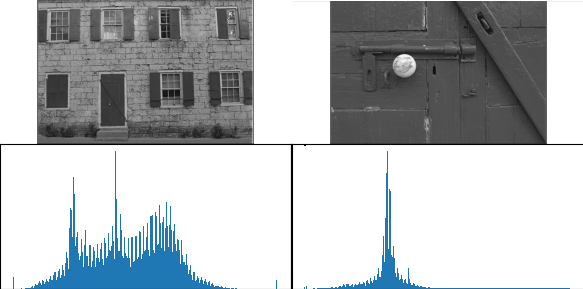
\includegraphics[width=0.9\textwidth]{img_hist.png}
    \caption{im\'agenes junto con sus histogramas de intensidad. Corresponden a las im\'agenes 1, 2, 13, y 22 del banco de im\'agenes.}
    \label{fig:img_hist}
\end{figure}

Podemos ver que cada histograma tiene una distribuci\'on distinta, algunas son se ven m\'as normales que otros, pero cabe notar que varias de est\'as fotos son multimodales, lo que dificulta el proceso de "normalizarlas", veamos ahora como se comportan las im\'agenes y su histograma al momento de aplicarles ruido. En la figura \ref{fig:img_hist_ruido} podemos ver las im\'agenes con ruido, junto con sus histogramas.

\begin{figure}[H]
    \centering
    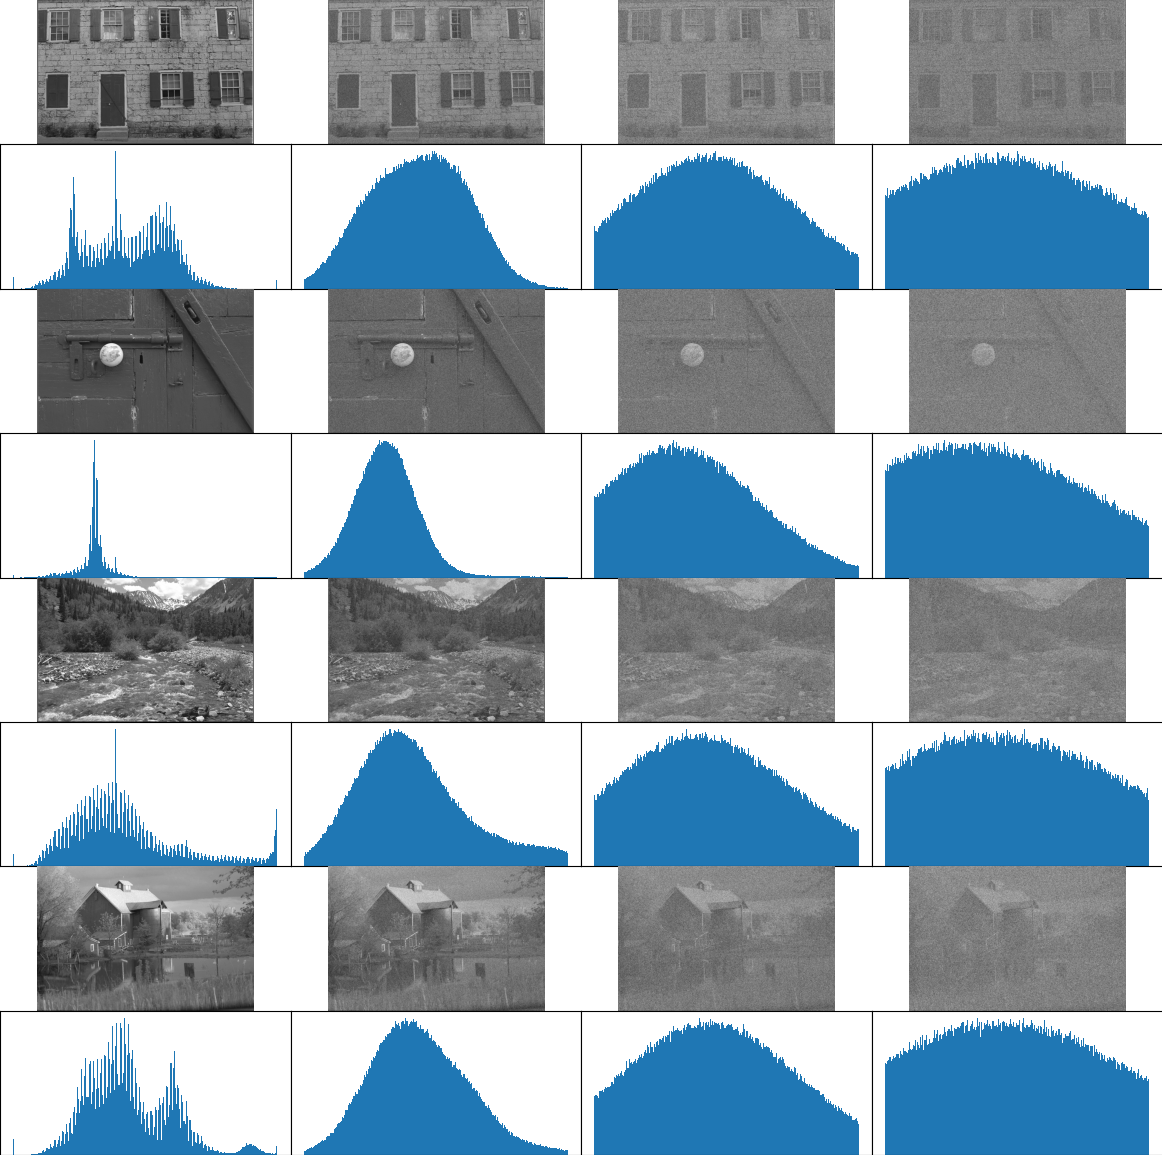
\includegraphics[width=0.9\textwidth]{img_hist_noise.png}
    \caption{im\'agenes junto con sus histogramas con ruido.}
    \label{fig:img_hist_ruido}
\end{figure}

Podemos ver que el ruido afecta de forma distinta a cada imagen, y que el histograma de cada imagen con ruido es distinto al histograma de la imagen original. Al momento de agregarles ruido gausiano es esperable que el histograma se vea más normal, y cabe destacar que la media de la distribución de los valores de intensidad queda centrada donde se encontraba la mayor moda del histograma original. 

Ahora, procederemos a revisar como se comporta la matriz de calor al ocmpara las im\'agenes con sus versiones con ruido. Recordemos que finalmente tenemos 4 m\'etodos propuestos de comparar las im\'agenes, por un lado tenemos MIC y dCor, y junto con esto en cada uno de ellos tenemos dos versiones, una donde comparamos directemente la imagen completa transformada a vector (recordemos que estos m\'etodos son agn\'osticos al orden), y otra donde comparamos los histogramas de las im\'agenes. Adem\'as incluimos el coeficientes de Pearson, utilizado de la misma forma. En la siguiente figura \ref{fig:heatmapall} podemos ver las matrices de calor para cada m\'etodo de comparaci\'on.

Notemos que la matrices para el resto de las im\'agenes se pueden encontrar en el Ap\'endice \ref{appA}

% do a figure with 4 images 
\begin{figure}[H]
    \centering
    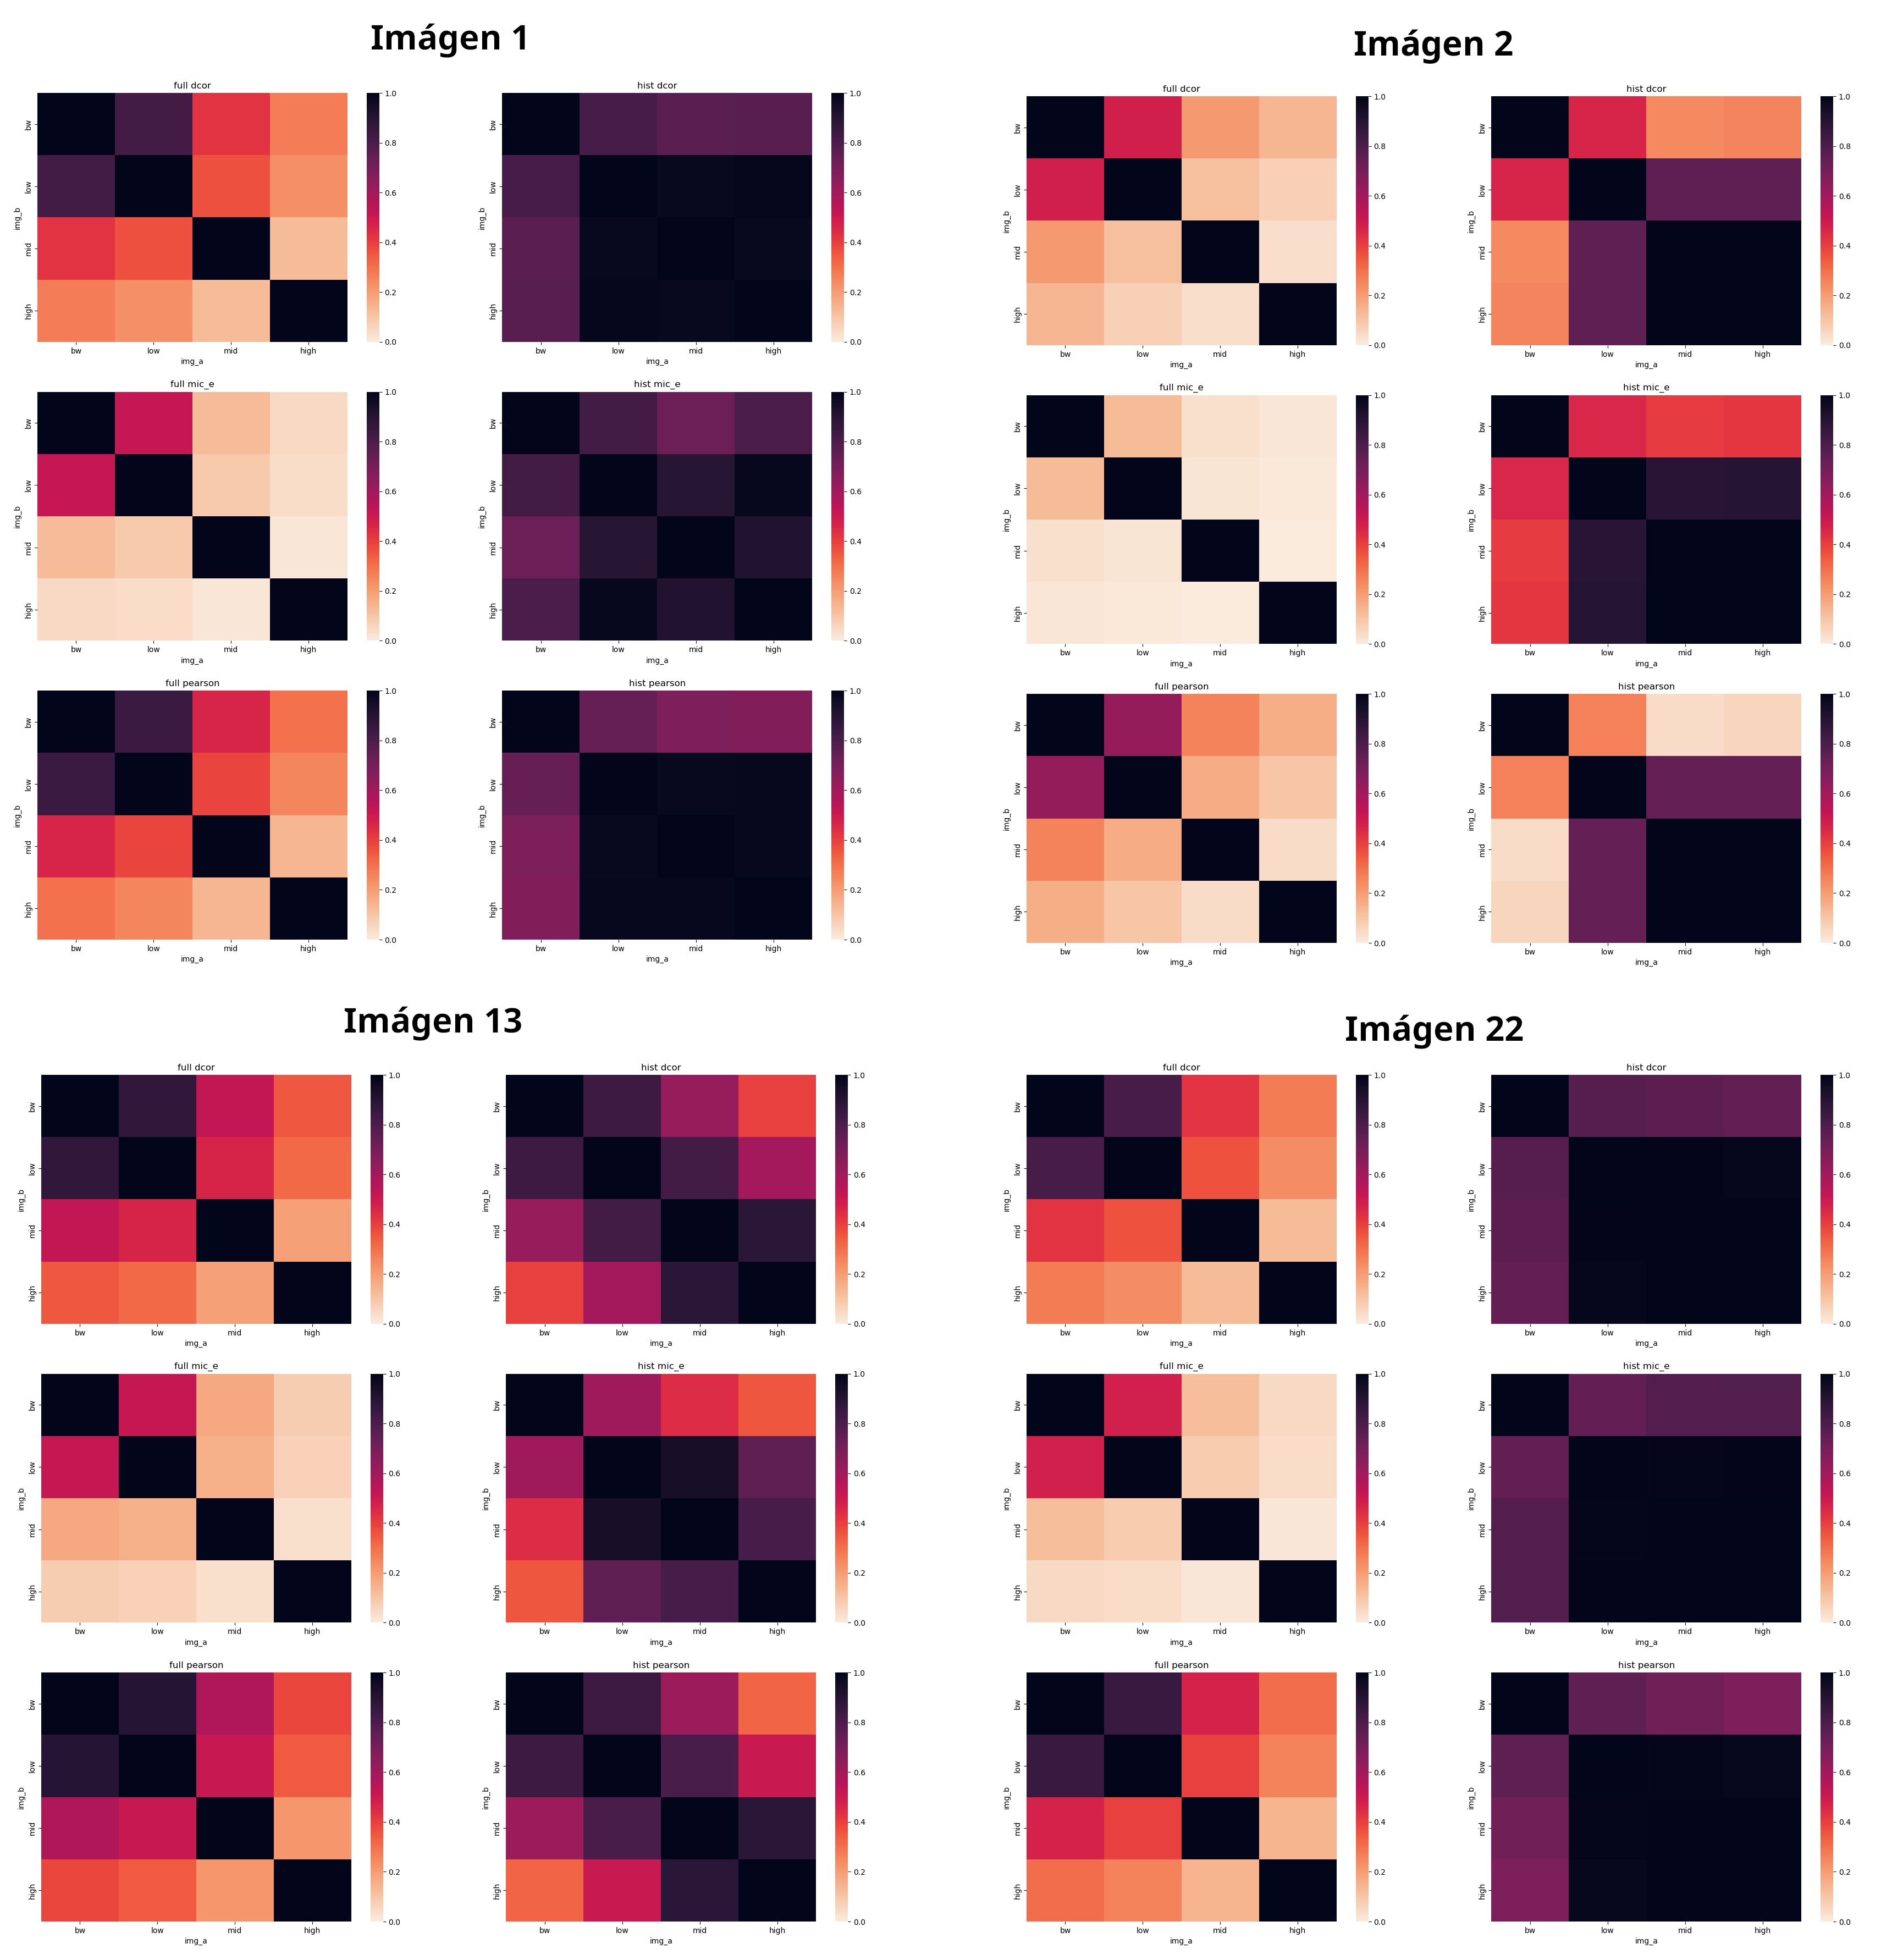
\includegraphics[width=0.95\textwidth]{heatmap_all.png}
    \caption{Matriz de calor para las im\'agenes 1, 2, 13, y 22 del banco, cada mapa de calor corresponde a un m\'etodo de comparaci\'on, ya sea comparando el total de la imagen (izquierda), o el histograma de estas (derecha). La cantidad de ruido aumenta de izquierda a derecha, y de arriba hacía abajo.}
    \label{fig:heatmapall}
\end{figure}

Notemos que a la izquierda tenemos la comparaci\'on del vector de las im\'agenes completo, y la derecha tenemos la comparaci\'on de los histogramas; además desde arriba hac\'ia abajo tenemos dCor, MIC, y Pearson.

Directamente podemos ver que existe una relaci\'on invesamente proporcional entre la cantidad de rudio y el coeficiente de comparaci\'on, lo que es esperable. Lo segundo que vale la pena mencionar es que en el caso de comparar los histogramas, en particular al momento de comparar entre las im\'agenes con ruidos obtenemos valores soprendentemente altos, esto es evidente al momento de ver la figura \ref{fig:img_hist_ruido}, donde podemos ver que los histogramas de las im\'agenes con ruido son bastante similares entre si. Pero si es destacable que se encontró una relaci\'on bastante fuerte entre los histogramas de las im\'agenes con ruido y las im\'agenes originales. 


Por ultimo vale la pena destcar que, en particular para el caso de la comparaci\'on del vector completo de la imagen, dCor y Pearson tienen un comportamiento bastante similar, mientras que MIC tiene dificultad para encontrar una relaci\'on entre las im\'agenes con niveles de ruido m\'as alto y la imagen original. 
